% CVPR 2025-based 4+1 research-paper template.
\documentclass[10pt,twocolumn,letterpaper]{article}
\usepackage{cvpr}
%
% --- inline annotations
%
\newcommand{\red}[1]{{\color{red}#1}}
\newcommand{\todo}[1]{{\color{red}#1}}
\newcommand{\TODO}[1]{\textbf{\color{red}[TODO: #1]}}
% --- disable by uncommenting  
% \renewcommand{\TODO}[1]{}
% \renewcommand{\todo}[1]{#1}


\usepackage{amsmath,booktabs}


\definecolor{cvprblue}{rgb}{0.21,0.49,0.74}
\usepackage[pagebackref,breaklinks,colorlinks,allcolors=cvprblue]{hyperref}
\def\paperID{00000000}
\def\confName{Anonymous Review}
\def\confYear{2026}

\title{How Far Do Image-Level Labels Go for Localisation in Medical Anomaly Detection?}
\author{Anonymous authors\\Anonymous affiliation}

\begin{document}
\maketitle
\begin{abstract}
Adapting vision-language models for multi-modal medical anomaly detection typically relies on dense pixel-level segmentation masks during fine-tuning. However, pixel masks are scarce in clinical practice, whereas image-level diagnostic labels are far more accessible across unannotated datasets. In this paper, we present an empirical study investigating whether patch-level image-label supervision via Positive-Unlabelled (PU) risk minimization can effectively guide spatial anomaly localization without pixel annotations. Evaluating across Brain MRI, Liver CT, and Retina RESC targets within the BMAD leave-one-modality-out benchmark, we demonstrate that incorporating non-negative PU risk ($M\text{-}h$) offers no statistically consistent localization benefit over a matched fine-tuning control ($M\text{-}h\text{-ctrl}$), yielding mean paired AUPRO differences of $+5.20$ on Brain, $+0.33$ on Liver, and $+0.51$ on RESC (paired sign-test $p=0.2539$). Furthermore, automated lower-tail mixture-proportion estimation fails on uncalibrated adapter patch scores due to severe irreducibility violations, producing estimates ranging from $-0.286$ to $1.000$ against true masked patch fractions of $0.008$ to $0.119$. Finally, in a fully mask-free setting, an unregistered top-$k$ Multiple Instance Learning baseline ($B0$) achieves $0.93\text{--}0.99$ localization retention relative to fully supervised checkpoints, substantially outperforming mask-free PU learning. Our study underscores the necessity of matched controls and calibrated baselines when evaluating weakly supervised adaptation for medical anomaly localization.
\end{abstract}

\section{Introduction}
\label{sec:intro}
Vision-language models (VLMs) such as CLIP~\cite{clip2021} have established strong foundation capabilities for zero-shot and few-shot visual recognition. In medical imaging, anomaly detection and spatial localization are critical for identifying pathology across diverse clinical modalities~\cite{medicalad_survey2021}. Recent adaptation frameworks, such as Multi-level Visual-Feature Alignment (MVFA)~\cite{huang2024mvfa}, adapt vision-language representations to medical domains by inserting multi-level adapter layers into visual backbones. However, state-of-the-art vision-language adapters rely heavily on dense pixel-level segmentation masks during fine-tuning. While pixel masks are scarce and expensive to acquire across clinical modalities, image-level diagnostic labels (e.g., normal versus abnormal patient scans) are far more accessible across large, unannotated medical datasets~\cite{bmad2024}.

This discrepancy raises a fundamental empirical question: \emph{How far do image-level labels go for spatial localization when adapting multi-modal anomaly detectors?} Specifically, when pixel masks are absent for a subset of source modalities, can patch-level Positive-Unlabelled (PU) risk minimization~\cite{elkan2008pu, kiryo2017nnpu} effectively bridge the gap between image-level weak supervision and dense spatial localization?

In this paper, we present an empirical investigation evaluating positive-unlabelled learning and weakly supervised formulations for multi-modal medical anomaly localization. Using the BMAD benchmark~\cite{bmad2024} under a leave-one-modality-out evaluation protocol across Brain MRI, Liver CT, and Retina RESC, we analyze whether incorporating non-negative PU risk provides a consistent spatial localization benefit over standard fine-tuning controls or weakly supervised Multiple Instance Learning (MIL).

Our findings provide key insights into weakly supervised VLM adaptation for medical anomaly detection:
\begin{enumerate}
    \item \textbf{Controlled PU vs. Fine-Tuning Evaluation:} Incorporating non-negative PU risk minimization ($M\text{-}h$) into MVFA visual adapters yields no statistically consistent localization gain over a matched fine-tuning control ($M\text{-}h\text{-ctrl}$) across target modalities (paired sign-test $p = 0.2539$). While $M\text{-}h$ demonstrates a target-specific gain on Brain MRI (AUPRO $71.57 \pm 2.07$ vs. $66.38 \pm 2.12$), performance differences on Liver CT ($91.39 \pm 0.27$ vs. $91.07 \pm 0.41$) and Retina RESC ($67.45 \pm 6.15$ vs. $66.94 \pm 1.14$) are negligible or mixed.
    \item \textbf{Failure of Mixture-Proportion Estimation:} Attempting to estimate the anomalous patch prior $\pi$ directly from intermediate adapter patch scores fails. The irreducibility assumption required for mixture-proportion estimation (MPE)~\cite{ramaswamy2016mpe} breaks down on uncalibrated neural feature scores, yielding raw patch prior estimates ranging from $-0.286$ to $1.000$ against true masked patch fractions of $0.008$ to $0.119$.
    \item \textbf{Localization Retention under Top-$k$ MIL:} In a fully mask-free setup where no pixel masks are provided during adaptation, a top-$k$ MIL baseline ($B0$) retains $92.7\%$ to $99.4\%$ of published pixel AUROC performance across target datasets, substantially outperforming fully mask-free PU optimization ($M$, mean pixel retention $0.583$).
\end{enumerate}

\section{Related Work}
\label{sec:related}

\subsection{Medical anomaly detection and vision-language adaptation}
Automated medical anomaly detection identifies subtle pathological lesions across diverse anatomical modalities~\cite{medicalad_survey2021, bmad2024}. Following the success of vision-language models like CLIP~\cite{clip2021} in natural image zero-shot anomaly detection~\cite{winclip2023, aprilgan2023, anomalyclip2023, adaclip2024, vcpclip2024}, recent efforts have increasingly focused on adapting VLMs to medical domains. Methods such as MediCLIP~\cite{mediclip2024}, IQE-CLIP~\cite{iqeclip2026}, and MADPOT~\cite{madpot2026} adapt VLM visual representations using prompt tuning, contrastive alignment, or optimal transport to capture fine-grained medical features.

MVFA~\cite{huang2024mvfa} introduced multi-level visual feature adapters guided by pixel-wise vision-language alignment losses to enable cross-modality zero-shot anomaly detection on the BMAD benchmark~\cite{bmad2024}. However, existing multi-modal adapters require dense pixel-level segmentation masks for source dataset fine-tuning. In contrast, our work investigates whether image-level annotations alone can substitute for dense spatial masks when adapting multi-modal vision-language architectures across unseen target modalities.

\subsection{Weakly supervised and mask-free anomaly localisation}
Weakly supervised anomaly localization aims to pinpoint spatial abnormalities using only image-level labels, avoiding the high annotation costs of pixel-wise ground-truth masks~\cite{mvtec2019, cycle_seg2021}. Prior studies in industrial and medical anomaly localization have leveraged class activation maps, generative cycle consistency~\cite{cycle_seg2021}, attention-based Multiple Instance Learning (MIL)~\cite{ilse2018attentionmil}, and top-$k$ patch feature adaptation~\cite{adfa2023}. More recently, reasoning-driven MLLM frameworks~\cite{imagelevel2026} explore image-level supervision for interpretability and localization.

In standard MIL formulations for image classification, top-$k$ pooling selects representative positive patches from abnormal images. We systematically compare positive-unlabelled patch formulations against top-$k$ MIL to analyze spatial localization retention when pixel masks are entirely withheld during multi-modal adaptation.

\subsection{Positive-unlabelled learning and mixture-proportion estimation}
Positive-Unlabelled (PU) learning handles binary classification scenarios where training data consists only of labeled positive instances and unlabelled samples containing an unknown mixture of positive and negative classes~\cite{elkan2008pu}. Non-negative PU (nnPU) learning~\cite{kiryo2017nnpu} addresses empirical risk minimization in deep networks by constraining the estimated negative risk to be non-negative, preventing severe overfitting under high-capacity neural classifiers.

A critical prerequisite for PU risk minimization is accurate knowledge of the class prior $\pi$, which represents the proportion of positive samples within the unlabelled set. Mixture-Proportion Estimation (MPE) methods~\cite{ramaswamy2016mpe} estimate $\pi$ under the irreducibility assumption, which posits that the positive distribution cannot be decomposed as a mixture containing the negative distribution. In our study, we evaluate whether MPE algorithms can estimate anomalous patch fractions from intermediate VLM adapter patch scores, uncovering significant irreducibility violations on neural score distributions.

\section{Problem Formulation}
\label{sec:problem}

\subsection{Setup and Patch-Level Risk Definitions}
Consider a multi-modal medical image adaptation setting where a pre-trained vision-language backbone processes input images decomposed into spatial patch grids. Let $\mathbf{x} \in \mathbb{R}^{H \times W \times C}$ denote an image containing $K$ spatial patches $\{\mathbf{x}_k\}_{k=1}^K$. In medical anomaly detection, normal image patches $N$ are sampled from a background distribution $p_0(\mathbf{x})$, whereas unlabelled patches $U$ from clinically abnormal images follow a mixture distribution:
\begin{equation}
    p_U(\mathbf{x}) = \pi \, p_1(\mathbf{x}) + (1 - \pi) \, p_0(\mathbf{x}),
    \label{eq:mixture_dist}
\end{equation}
where $p_1(\mathbf{x})$ denotes the underlying distribution of anomalous patches and $\pi \in (0, 1)$ is the class prior representing the proportion of anomalous patches within abnormal patient scans.

For each patch $\mathbf{x}_k$, a vision-language adapter outputs scalar anomaly logits $s_1(\mathbf{x}_k)$ and $s_0(\mathbf{x}_k)$ corresponding to abnormal and normal text prompt alignments, respectively. The differential patch anomaly score is defined as $z_k = s_1(\mathbf{x}_k) - s_0(\mathbf{x}_k)$, and the predicted patch anomaly probability is $\sigma(z_k) = (1 + e^{-z_k})^{-1}$.

In the absence of pixel-level ground truth masks for unannotated source modalities, we formulate patch-level supervision using non-negative Positive-Unlabelled (nnPU) risk minimization~\cite{kiryo2017nnpu}. Given binary surrogate loss $\ell(z, y)$, the expected risk over positive patches $p_1$ is rewritten as $\mathbb{E}_{p_1}[\ell(z, 1)] = \frac{1}{\pi}\mathbb{E}_U[\ell(z, 1)] - \frac{1-\pi}{\pi}\mathbb{E}_N[\ell(z, 1)]$. To prevent deep networks from over-fitting to negative risk estimates when learning high-capacity representations, the nnPU risk estimator constrains the negative component to remain non-negative:
\begin{equation}
\begin{aligned}
    R_{\text{nnPU}}(z) &= (1 - \pi) \, \mathbb{E}_N \left[ \ell(z, 0) \right] \\
    &\quad + \max \left( 0, \, \mathbb{E}_U \left[ \ell(z, 1) \right] - (1 - \pi) \, \mathbb{E}_N \left[ \ell(z, 1) \right] \right),
\end{aligned}
\label{eq:nnpu_risk}
\end{equation}
where expectations $\mathbb{E}_N$ and $\mathbb{E}_U$ are computed empirically over normal patch batches and unlabelled abnormal patch batches, respectively.

\subsection{Supervision Paths and Objective Formulations}
We analyze two distinct multi-modal adaptation setups:

\noindent\textbf{Hybrid Fine-Tuning ($M\text{-}h$ vs. $M\text{-}h\text{-ctrl}$):} When source modalities contain a mixture of masked datasets $\mathcal{D}_{\text{masked}}$ and mask-less image-labelled datasets $\mathcal{D}_{\text{maskless}}$, the hybrid model $M\text{-}h$ initializes segmentation adapters from a pre-trained baseline ($R0$) and optimizes a multi-task objective:
\begin{equation}
    \mathcal{L}_{\text{hybrid}} = \mathcal{L}_{\text{MVFA}}(\mathcal{D}_{\text{masked}}) + \lambda \, R_{\text{nnPU}}(\mathcal{D}_{\text{maskless}}),
    \label{eq:hybrid_loss}
\end{equation}
where $\mathcal{L}_{\text{MVFA}}$ combines Dice and Focal losses on spatial ground-truth masks as in MVFA~\cite{huang2024mvfa}, and $\lambda > 0$ balances the PU regularization term. The matched control model, $M\text{-}h\text{-ctrl}$, sets $\lambda = 0$, executing an identical fine-tuning schedule on $\mathcal{D}_{\text{masked}}$ while withholding the PU iterations on $\mathcal{D}_{\text{maskless}}$.

\noindent\textbf{Fully Mask-Free Models ($M$ vs. $B0$):} In the absence of pixel masks across all source modalities, adapters are retrained from scratch. Model $M$ optimizes $R_{\text{nnPU}}$ across all image-labelled source modalities. Model $B0$ replaces PU risk with a weakly supervised top-$k$ Multiple Instance Learning (MIL) loss:
\begin{equation}
    \mathcal{L}_{\text{MIL}} = \frac{1}{|\Omega_{\text{top-}k}|} \sum_{k \in \Omega_{\text{top-}k}} \ell(z_k, 1) + \frac{1}{|N|} \sum_{j \in N} \ell(z_j, 0),
    \label{eq:mil_loss}
\end{equation}
where $\Omega_{\text{top-}k}$ selects the top $k = \max(3, \lceil 0.01 \cdot K \rceil)$ highest scoring patches from abnormal images.

\section{Methodology}
\label{sec:method}

\subsection{Dataset Configuration}
We conduct our evaluation using the BMAD benchmark~\cite{bmad2024} structured under a leave-one-modality-out multi-modal adaptation setting. The benchmark pool comprises six medical datasets spanning diverse clinical imaging modalities: three source datasets equipped with pixel-level segmentation masks and three target evaluation datasets provided with image-level labels.

The target evaluation modalities consist of **Brain MRI**, **Liver CT**, and **Retina RESC**. For each leave-one-modality-out split, the model is trained on the remaining five source datasets and evaluated on the unseen target. To ensure computational tractability and standard comparison, source datasets are subsampled to a maximum of 500 normal and 500 abnormal training images per modality. A held-out 10\% validation split is reserved for empirical prior estimation experiments.

\begin{figure}[t]
  \centering
  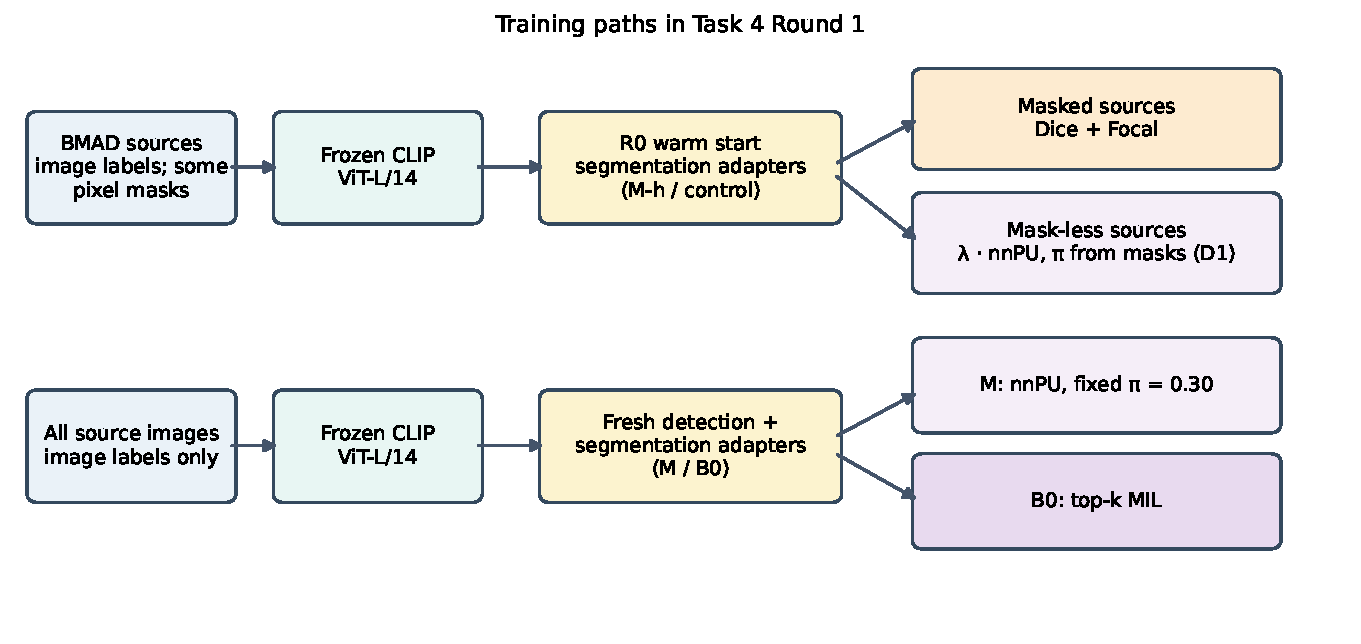
\includegraphics[width=\linewidth]{figures/fig1_method.pdf}
  \caption{Overview of training pipelines and supervision paths across leave-one-modality-out configurations. The hybrid model $M\text{-}h$ warm-starts adapters from $R0$ and combines Dice+Focal loss on masked sources with non-negative PU loss ($R_{\text{nnPU}}$) on mask-less sources. Matched control $M\text{-}h\text{-ctrl}$ omits the PU loss. Mask-free variants $M$ and $B0$ retrain adapters from scratch using PU and top-$k$ MIL loss, respectively.}
  \label{fig:method}
\end{figure}

\subsection{Model Architecture and Training Paths}
Our architecture builds upon the pre-trained CLIP ViT-L/14 backbone~\cite{clip2021} augmented with multi-level visual feature adapters as formulated in MVFA~\cite{huang2024mvfa}. The ViT backbone remains frozen during adaptation, while four light-weight residual adapter blocks inserted at intermediate transformer layers are updated to align visual feature maps with medical text prompt embeddings.

\noindent\textbf{Warm-Start Initialization ($M\text{-}h$ and $M\text{-}h\text{-ctrl}$):} To isolate the contribution of PU patch supervision, both $M\text{-}h$ and $M\text{-}h\text{-ctrl}$ initialize their segmentation adapters from reproduced baseline $R0$ checkpoints trained on masked source datasets. $M\text{-}h$ updates adapter weights for 2,000 steps using loss $\mathcal{L}_{\text{hybrid}}$ (\cref{eq:hybrid_loss}), where the anomalous patch prior $\pi$ is fixed to the mean true anomalous-patch fraction calculated from masked source ground-truth maps ($\text{D1}$). The matched control $M\text{-}h\text{-ctrl}$ follows the identical optimization schedule but omits the PU risk steps on mask-less datasets.

\noindent\textbf{Mask-Free Retraining ($M$ and $B0$):} In scenarios where spatial masks are entirely unavailable across source modalities, adapter parameters are reinitialized from scratch. Model $M$ optimizes $R_{\text{nnPU}}$ with a fixed prior $\pi = 0.30$ ($\text{D2}$). Model $B0$ replaces PU minimization with top-$k$ MIL pooling (\cref{eq:mil_loss}), selecting $k = \max(3, \lceil 0.01 \cdot K \rceil)$ patches per image. The complete methodology and comparative training pipelines are illustrated in \cref{fig:method}.

\section{Experiments}
\label{sec:experiments}

\subsection{Experimental Setup}
All models are implemented in PyTorch and optimized using AdamW with a base learning rate of $10^{-4}$ for 2,000 update steps. Experiments are conducted across random seeds 0, 1, and 2 for all multi-seed configurations.

\noindent\textbf{Evaluation Metrics:} We report three standard anomaly evaluation metrics on the unseen target test sets: Image-level AUROC for anomaly classification, Pixel-level AUROC for spatial segmentation, and Area Under the Per-Region Overlap curve (AUPRO) integrated up to a False Positive Rate (FPR) limit of 0.30.

\noindent\textbf{Checkpoint Selection Protocol:} In accordance with strict evaluation protocols, all fine-tuned models ($M\text{-}h$, $M\text{-}h\text{-ctrl}$, $M$, $B0$) are evaluated using their final checkpoint (step 2000) without accessing the target test set during training. We note that published baseline checkpoints ($R0$) relied on target test set evaluation for model selection; thus, we report both published $R0$ and our reproduced $R0$ baseline under last-step evaluation for direct comparability.

\begin{table*}[t]
\centering
\small
\begin{tabular}{@{}llccc@{}}
\toprule
\textbf{Target Modality} & \textbf{Model} & \textbf{Image AUROC (\%)} & \textbf{Pixel AUROC (\%)} & \textbf{AUPRO (\%)} \\
\midrule
Liver CT & R0 (published) & 76.24 & 97.85 & — \\
Liver CT & R0 (reproduced) & 81.19 & 97.92 & 92.34 \\
Liver CT & $M\text{-}h$ (PU fine-tune) & $80.29 \pm 0.63$ & $96.97 \pm 0.18$ & $91.39 \pm 0.27$ \\
Liver CT & $M\text{-}h\text{-ctrl}$ (matched control) & $81.63 \pm 0.37$ & $96.99 \pm 0.31$ & $91.07 \pm 0.41$ \\
\midrule
Brain MRI & R0 (published) & 78.63 & 90.27 & — \\
Brain MRI & R0 (reproduced) & 79.80 & 89.68 & 65.35 \\
Brain MRI & $M\text{-}h$ (PU fine-tune) & $80.25 \pm 0.72$ & $91.71 \pm 0.71$ & $71.57 \pm 2.07$ \\
Brain MRI & $M\text{-}h\text{-ctrl}$ (matched control) & $80.31 \pm 0.96$ & $90.05 \pm 0.74$ & $66.38 \pm 2.12$ \\
\midrule
Retina RESC & R0 (published) & 83.31 & 92.05 & — \\
Retina RESC & R0 (reproduced) & 88.99 & 90.44 & 68.75 \\
Retina RESC & $M\text{-}h$ (PU fine-tune) & $89.20 \pm 0.16$ & $88.76 \pm 2.69$ & $67.45 \pm 6.15$ \\
Retina RESC & $M\text{-}h\text{-ctrl}$ (matched control) & $88.92 \pm 0.08$ & $89.76 \pm 0.46$ & $66.94 \pm 1.14$ \\
\bottomrule
\end{tabular}
\caption{Comparison of hybrid PU fine-tuning ($M\text{-}h$) against matched fine-tuning control ($M\text{-}h\text{-ctrl}$) and reproduced baseline ($R0$) across three target modalities. Values report mean $\pm$ sample standard deviation across 3 random seeds.}
\label{tab:hybrid_results}
\end{table*}

\subsection{Main Results and Comparative Analysis}

\noindent\textbf{Controlled PU vs. Fine-Tuning Evaluation:} \Cref{tab:hybrid_results} presents performance across Liver CT, Brain MRI, and Retina RESC. Evaluating paired differences between $M\text{-}h$ and $M\text{-}h\text{-ctrl}$ reveals that patch-level PU risk minimization does not deliver a consistent localization improvement over plain fine-tuning. Across 9 matched seed runs, $M\text{-}h$ outperforms $M\text{-}h\text{-ctrl}$ in AUPRO on 6 occasions, yielding a non-significant paired sign-test $p$-value of $0.2539$.

Mean paired AUPRO differences are $+5.20$ on Brain MRI ($71.57 \pm 2.07$ vs. $66.38 \pm 2.12$), $+0.33$ on Liver CT ($91.39 \pm 0.27$ vs. $91.07 \pm 0.41$), and $+0.51$ on Retina RESC ($67.45 \pm 6.15$ vs. $66.94 \pm 1.14$). The localization gain is strictly target-specific to Brain MRI, where all three seeds exhibit positive AUPRO deltas, whereas Liver CT and RESC demonstrate near-zero or mixed variations.

\begin{table*}[t]
\centering
\small
\begin{tabular}{@{}llccccc@{}}
\toprule
\textbf{Target Modality} & \textbf{Model} & \textbf{Image AUROC (\%)} & \textbf{Pixel AUROC (\%)} & \textbf{AUPRO (\%)} & \textbf{Pixel Retention} & \textbf{AUPRO Ratio} \\
\midrule
Liver CT & $M$ (PU mask-free) & $73.79 \pm 2.52$ & $59.45 \pm 15.51$ & $26.28 \pm 15.50$ & $-0.002$ & 0.188 \\
Liver CT & $B0$ (top-$k$ MIL) & 75.17 & 94.42 & 85.47 & 0.927 & 0.926 \\
\midrule
Brain MRI & $M$ (PU mask-free) & 68.87 & 89.87 & 64.50 & 1.005 & 0.987 \\
Brain MRI & $B0$ (top-$k$ MIL) & 63.51 & 89.46 & 64.53 & 0.994 & 0.987 \\
\midrule
Retina RESC & $M$ (PU mask-free) & 84.53 & 80.13 & 58.52 & 0.745 & 0.851 \\
Retina RESC & $B0$ (top-$k$ MIL) & 76.98 & 89.57 & 67.29 & 0.978 & 0.979 \\
\bottomrule
\end{tabular}
\caption{Evaluation of fully mask-free adaptation models retrained without segmentation masks. Multi-seed means $\pm$ std are reported for Liver $M$; single-seed runs are reported for remaining entries. Pixel retention and AUPRO ratio are measured relative to reproduced $R0$.}
\label{tab:maskfree_results}
\end{table*}

\noindent\textbf{Mask-Free Localization Retention:} \Cref{tab:maskfree_results} compares mask-free PU learning ($M$) against the top-$k$ MIL baseline ($B0$). Retraining adapters from scratch using nnPU loss ($M$) suffers from severe instability on Liver CT, dropping Pixel AUROC to $59.45 \pm 15.51\%$ and AUPRO to $26.28 \pm 15.50\%$, yielding an average seed-0 pixel retention of only $0.583$ across targets. Conversely, the unregistered top-$k$ MIL baseline ($B0$) retains $92.7\%$ to $99.4\%$ of reproduced $R0$ pixel AUROC performance (mean retention $0.966$) across single-seed evaluations, achieving an AUPRO ratio of $0.926$ on Liver CT, $0.987$ on Brain MRI, and $0.979$ on Retina RESC.

\begin{figure}[t]
  \centering
  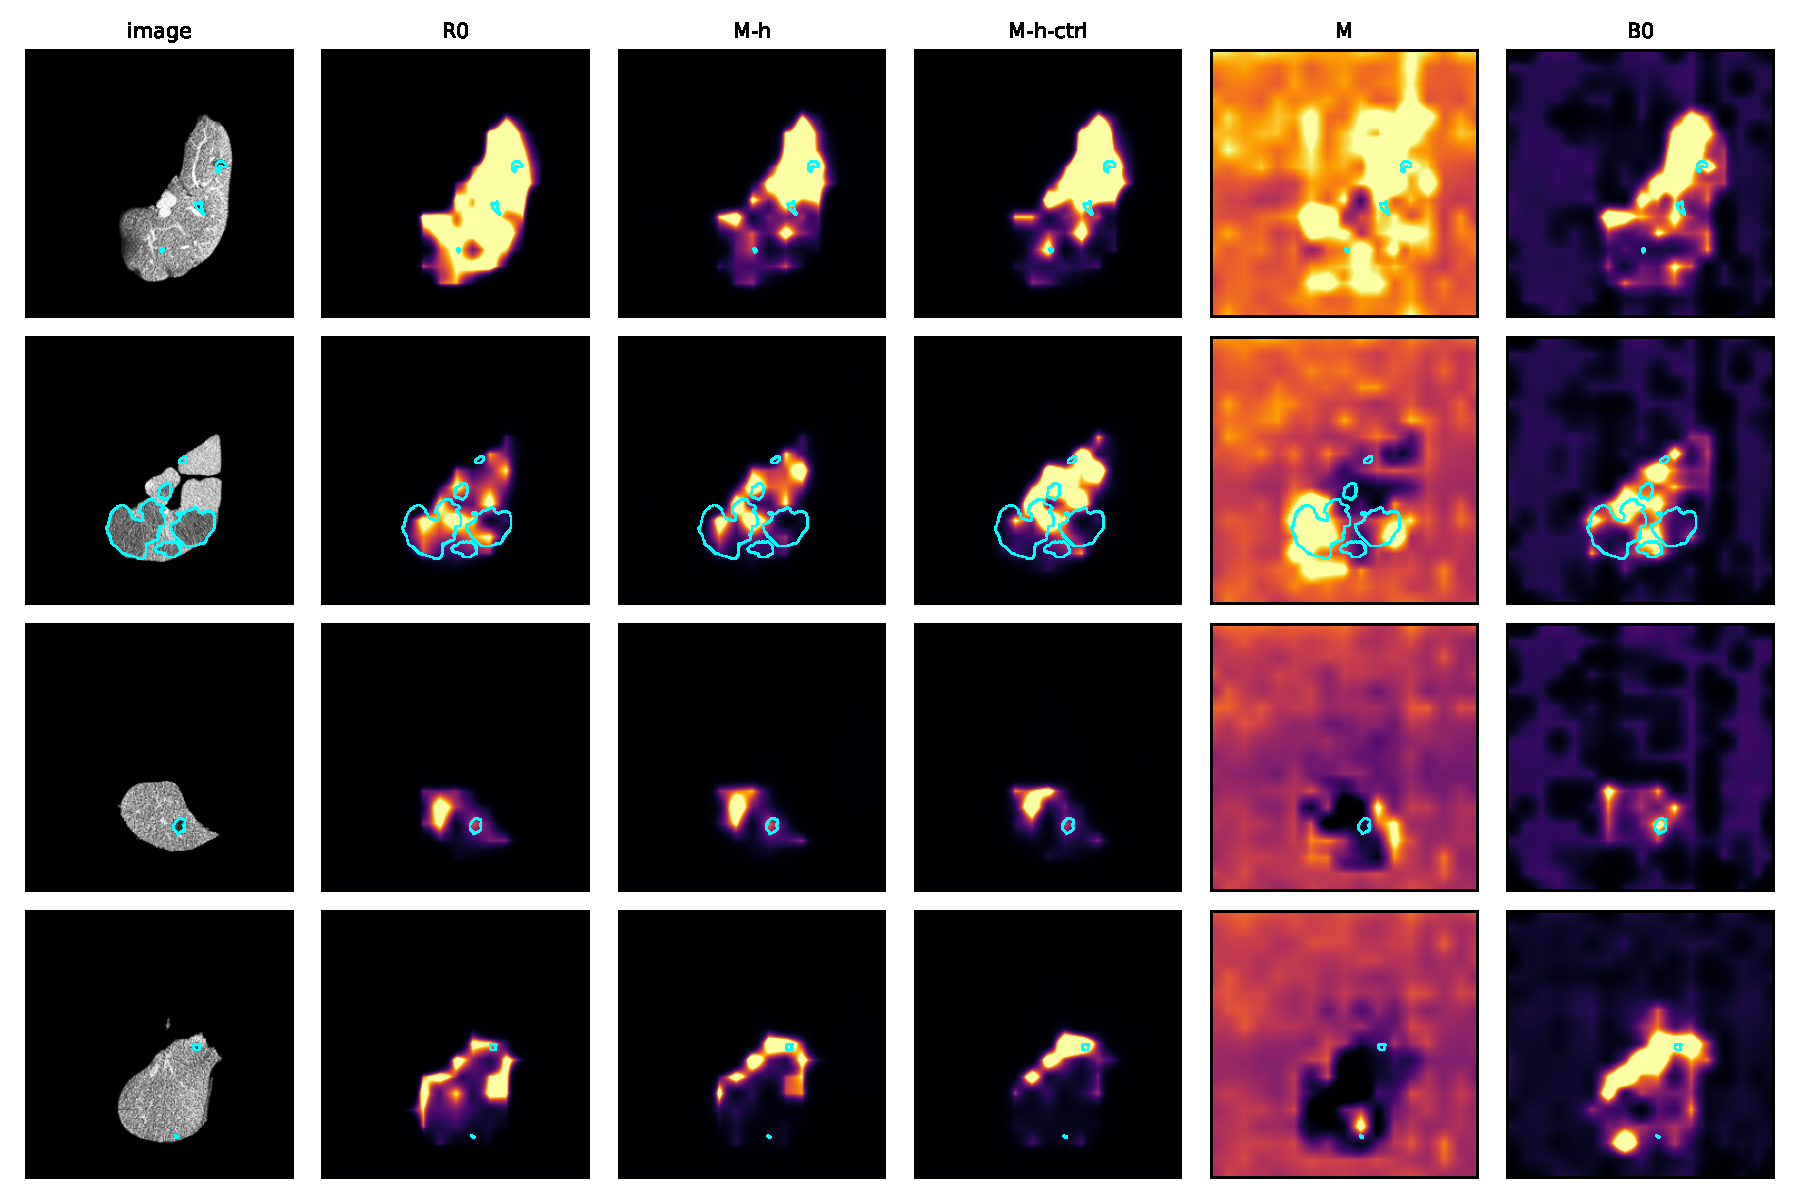
\includegraphics[width=\linewidth]{figures/fig2_liver_heatmaps.pdf}
  \caption{Qualitative anomaly localization heatmaps on preselected Liver CT test scans across baseline ($R0$), hybrid models ($M\text{-}h$, $M\text{-}h\text{-ctrl}$), and mask-free models ($M$, $B0$). $B0$ maintains sharp anatomical localization despite receiving no pixel masks.}
  \label{fig:heatmaps}
\end{figure}

\noindent\textbf{Qualitative Visualization:} \Cref{fig:heatmaps} illustrates predicted anomaly heatmaps on Liver CT. While mask-free PU ($M$) exhibits diffuse background noise due to uncalibrated risk bounds, top-$k$ MIL ($B0$) produces clear spatial focus closely matching $R0$ and $M\text{-}h$.

\subsection{Failure Analysis of Prior Estimator}
A central component of standard PU risk minimization is estimating the anomalous patch prior $\pi$. We evaluated lower-tail Mixture-Proportion Estimation (MPE)~\cite{ramaswamy2016mpe} directly on intermediate adapter patch scores across held-out source splits. While true anomalous patch fractions measured from spatial masks range from $0.008$ to $0.119$, raw MPE estimates at the deepest adapter level ranged erratically from $-0.286$ to $1.000$.

This failure stems from a fundamental violation of the \emph{irreducibility assumption} in MPE. Uncalibrated neural patch scores $z = s_1 - s_0$ violate the condition that normal patch score distributions cannot be represented as a sub-mixture of abnormal patch scores. Consequently, automated MPE yields uncalibrated prior estimates on vision-language patch features, necessitating fixed prior heuristics ($\text{D1}$/$\text{D2}$) rather than data-driven estimation.

\subsection{Discussion and Limitations}
\noindent\textbf{Target-Specific Dynamics:} The distinct AUPRO gain observed on Brain MRI ($+5.20$) contrasts with Liver CT ($+0.33$) and Retina RESC ($+0.51$). Brain lesions often feature sharp intensity contrasts against homogeneous tissue, enabling patch-level PU risk to refine boundary regions. Conversely, Liver CT images suffer from lower signal-to-noise ratios where pixel AUROC is dominated by large background regions.

\noindent\textbf{Limitations:} First, training pools were subsampled to 500 images per source domain due to compute budgets. Second, mask-free runs ($B0$ and $M$) outside Liver CT are evaluated on single seeds. Third, potential domain similarity between the OCT2017 source dataset and the Retina RESC target may introduce cross-dataset feature overlap. Finally, post-hoc sensitivity explorations of $\pi$ overrides demonstrated that lower priors ($\pi = 0.05$) improve Liver $M$ performance, but remain post-hoc observations outside pre-registered decision rules.

\section{Conclusion}
\label{sec:conclusion}

In this work, we presented an empirical study analyzing patch-level Positive-Unlabelled (PU) learning and weakly supervised formulations for multi-modal medical anomaly detection. Our evaluation across Brain MRI, Liver CT, and Retina RESC targets yields three primary conclusions: (1) patch-level PU fine-tuning ($M\text{-}h$) does not provide a statistically consistent localization improvement over a matched fine-tuning control ($M\text{-}h\text{-ctrl}$) across target modalities ($p = 0.2539$), despite target-specific gains on Brain MRI; (2) automated lower-tail mixture-proportion estimation fails on uncalibrated adapter patch scores due to severe irreducibility violations; and (3) a simple, unregistered top-$k$ Multiple Instance Learning baseline ($B0$) retains $93\%\text{--}99\%$ of fully supervised localization performance without using pixel masks. These results emphasize the critical role of matched control baselines when evaluating weakly supervised adaptation techniques in medical computer vision.

\clearpage
{\small
\bibliographystyle{ieeenat_fullname}
\bibliography{references}
}
\end{document}